\newpage
\section{Auswertung}
\label{sec:Auswertung}
\subsection{Eichung des Magnetfeldes}
\label{sec:eich}
Die bei der Messung aufgenommenen Magnetfeldstärken $B$ bei angelegter Stromstärke $I$ befinden sich in Tabelle \ref{tab:bfeld}.

\begin{table}
    \centering
    \sisetup{table-format=2.1}
    \begin{tabular}{c c}
    \toprule
    $I \,/\,A$ & $B \,/\, mT$ \\
     \midrule 
  0  & 7.6  \\
  0.5  & 60  \\
  1  & 105.6   \\
  1.5  & 154.1  \\
  2  & 202.3   \\
  2.5  & 255.1  \\
  3  & 298.6   \\
  3.5  & 339.1  \\
  4  &  386.2   \\
  4.5  &  421.3 \\
  5  & 455.7 \\
    \bottomrule
    \end{tabular}
    \caption{Messwerte der Magnetfeldstärke in Abhängigkeit der Stromstärke.}
    \label{tab:bfeld}
    \end{table}


\noindent
Die Messwerte werden mittels der Funktion curve\_fit aus dem Paket scipy.optimize in Python an eine Funktion dritten Grades gefittet.
Für die Fitfunktion

\begin{equation*}
    B(I)=aI^3 + bI^2 + cI + d
\end{equation*}

\noindent
werden die folgenden Parameter ermittelt:

\begin{align*}
    a&=-0.78 \pm 0.25 \, \frac{\text{mT}}{\text{A}^3} \\
    b&=2.70  \pm 1.90 \, \frac{\text{mT}}{\text{A}^2} \\
    c&=95.34 \pm 3.97 \, \frac{\text{mT}}{\text{A}} \\
    d&=8.90  \pm 2.18 \, \text{mT} \\
\end{align*}

\noindent
Die Messwerte und die Ausgleichskurve sind in Abbildung \ref{fig:bfeld} dargestellt.

\begin{figure}
    \centering
    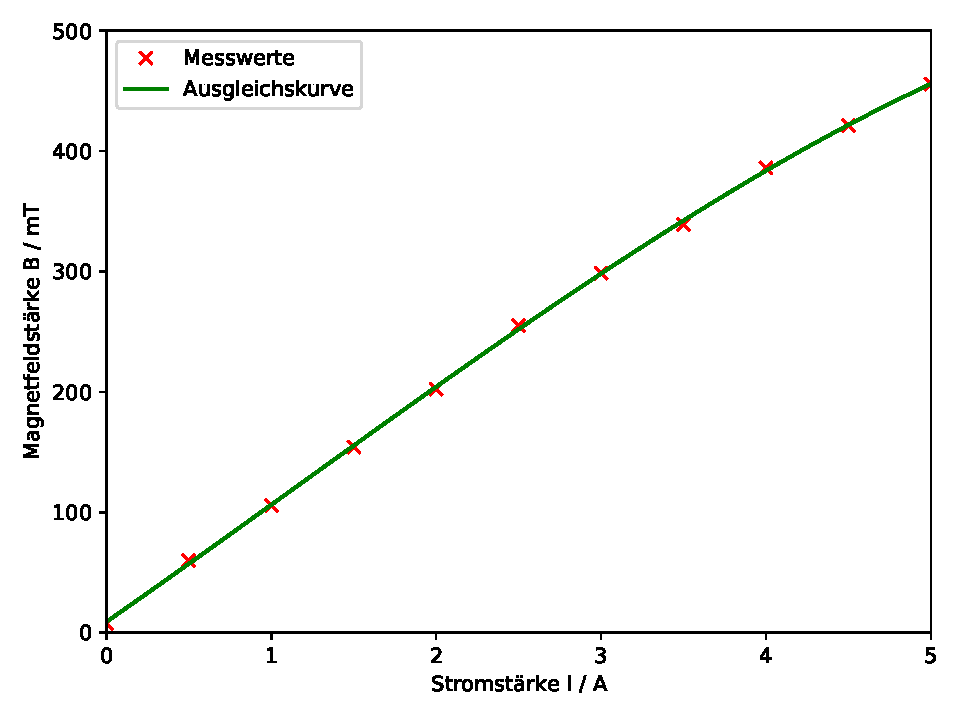
\includegraphics[width=0.75\textwidth]{data/Magnetfeld.pdf}
    \caption{Ausgleichskurve durch die Messwerte der Magnetfeldstärke.}
    \label{fig:bfeld}
  \end{figure}

\newpage
\subsection{Rote Spektrallinie}
In Abbildung \ref{fig:rot} sind die Interferenzmuster der Spektrallinie der Wellenlänge $\lambda = 643$nm einer Cd-Lampe dargestellt.
Dabei wurde Abbildung \ref{fig:rot1} ohne äußeres Magnetfeld aufgenommen.
Bei der Aufnahme von Abbildung \ref{fig:rot1b} wurden die Elektromagneten mit einer maximalen Stromstärke von $I=5$ A betrieben, was nach der Eichung aus Kapitel \ref{sec:eich} einem Magnetfeld von $B= 455.87 \pm 60.21$ mT entspricht.
Durch die Verwendung eines Polarisationsfilters wird nur die Emission des $\sigma$-Übergangs beobachtet.
Die Abstände der Interferenzmaxima $\Delta s$ ohne B-Feld und $\delta s$ mit B-Feld in Pixeln befinden sich in Tabelle \ref{tab:rot}.


\noindent
Da die Abstände manuell abgelesen wurden, wird eine Unsicherheit von $x=10$ px für alle Messwerte angenommen.


\begin{figure}[H]
	\centering
	\begin{subfigure}[b]{0.8\textwidth}
		\centering
		
\includegraphics[width=0.8\textwidth]{data/rot1.JPG}
		\caption{Ohne Magnetfeld.}
    \label{fig:rot1}
	\end{subfigure}
	
	\begin{subfigure}[b]{0.8\textwidth}
		\centering
		
\includegraphics[width=0.8\textwidth]{data/rot1b.JPG}
		\caption{Magnetfeld von $B= 455.87$ mT.}
    \label{fig:rot1b}
	\end{subfigure}
    \caption{Interferenzmuster der roten Spektrallinie einer Cd-Lampe.}
\label{fig:rot}
\end{figure}


\begin{table}
    \centering
    \sisetup{table-format=2.1}
    \begin{tabular}{c c c}
    \toprule
    $\text{Ordnung}$ & $\Delta s \,/\, \text{px}$ & $\delta s \,/\, \text{px}$ \\
     \midrule 
     1 &  235 & 78 \\
     2 &  237 & 76\\
     3 &  238 & 86\\
     4 &  236 & 81\\
     5 &  243 & 80\\
     6 &  248 & 86\\
     7 &  251 & 84\\
     8 &  245 & 84\\
     9 &  247 & 83\\
     10 &  255 & 86\\
    \bottomrule
    \end{tabular}
    \caption{Abstände der Interferenzmaxima der roten Spektrallinie.}
    \label{tab:rot}
    \end{table}

\newpage
\noindent
Mit der Formel 

\begin{equation}
  \label{eqn:Wellenlaenge}
  \delta \lambda = \frac{1}{2} \frac{\delta s}{\Delta s} \cdot \lambda_D
\end{equation}

\noindent
und den Werten aus Tabelle \ref{tab:rot} sowie dem Dispersionsgebiet $\lambda_D = 48.91$ pm nach Formel \ref{eqn:lam}, kann nun die Wellenlängenverschiebung 

\begin{equation*}
    \delta \lambda = 8.28 \pm 0.34 \, \text{pm}
  \end{equation*}

\noindent
berechnet werden. Wird nun die Energiedifferenz

\begin{equation}
    |\Delta E| \approx \left | \frac{\delta E}{\delta \lambda} \right | \cdot |\delta \lambda | = \frac{h c}{\lambda^2} \cdot \delta \lambda
\end{equation}

\noindent
in Gleichung \ref{eqn:anorm} eingesetzt, kann der Landé-Faktor mit 

\begin{equation}
    \label{eqn:g}
    g = \delta \lambda \frac{hc}{\mu_B B \lambda^2}.
\end{equation}

\noindent
bestimmt werden. Somit ergibt sich für die rote $\sigma$-Spektrallinie

\begin{center}
    $g_{Rot} = 0.94 \pm 0.04$.
\end{center}

\noindent
Wird der Polarisationsfilter so gedreht, dass die $\pi$-Übergänge beobachtet werden, entstehen die Interferenzmuster aus Abbildung \ref{fig:rot22}.

\begin{figure}[H]
	\centering
	\begin{subfigure}[b]{0.8\textwidth}
		\centering
		
\includegraphics[width=0.8\textwidth]{data/rot2.JPG}
		\caption{Ohne Magnetfeld.}
    \label{fig:rot1}
	\end{subfigure}
	
	\begin{subfigure}[b]{0.8\textwidth}
		\centering
		
\includegraphics[width=0.8\textwidth]{data/rot2b.JPG}
		\caption{Magnetfeld von $B= 455.87$ mT.}
    \label{fig:rot1b}
	\end{subfigure}
    \caption{Interferenzmuster der roten Spektrallinie einer Cd-Lampe.}
\label{fig:rot22}
\end{figure}

\noindent
Wie in Kapitel \ref{sec:durch}
bereits diskutiert wurde, ist bei dem $\pi$-Übergang der roten Spektrallinie keine Aufspaltung zu erwarten.

\subsection{Blaue Spektralinie}
In Abbildung \ref{fig:blau} sind die Interferenzmuster für die Spektralinie der Wellenlänge $\lambda=480$ nm dargestellt, 
wobei aufgrund des Polarisationsfilters nur die Emission des $\sigma$-Übergangs beobachtet wird.
Die Stromstärke an den Elektromagneten beträgt $I=3.2$ A, was nach Kapitel \ref{sec:eich} einem Magnetfeld von $B = 316.16 \pm 24.72$ mT entspricht.
Die bestimmten Abstände mit der Unsicherheit $x=10$ px befinden sich in Tabelle \ref{tab:blau}.


\begin{figure}[H]
	\centering
	\begin{subfigure}[b]{0.8\textwidth}
		\centering
		
\includegraphics[width=0.8\textwidth]{data/blau1.JPG}
		\caption{Ohne Magnetfeld.}
    \label{fig:blau1}
	\end{subfigure}
	
	\begin{subfigure}[b]{0.8\textwidth}
		\centering
		
\includegraphics[width=0.8\textwidth]{data/blau1b.JPG}
		\caption{Magnetfeld von $B= 316.16$ mT.}
    \label{fig:rot1b}
	\end{subfigure}
    \caption{Interferenzmuster der blauen Spektrallinie einer Cd-Lampe.}
\label{fig:blau}
\end{figure}


\begin{table}
    \centering
    \sisetup{table-format=2.1}
    \begin{tabular}{c c c}
    \toprule
    $\text{Ordnung}$ & $\Delta s \,/\, \text{px}$ & $\delta s \,/\, \text{px}$ \\
     \midrule 
     1 & 134 & 47 \\
     2 & 129 & 42 \\
     3 & 133 & 43 \\
     4 & 131 & 44 \\
     5 & 130 & 46 \\
     6 & 131 & 48 \\
     7 & 133 & 46 \\
     8 & 128 & 43 \\
     9 & 129 & 45 \\
     10 & 131 & 49 \\
    \bottomrule
    \end{tabular}
    \caption{Abstände der Interferenzmaxima der blauen Spektrallinie.}
    \label{tab:blau}
    \end{table}

    \noindent
    Mit dem Dispersionsgebiet $\lambda_D = 26.95$ pm und Formel \ref{eqn:Wellenlaenge} ergibt sich für die Wellenlängenverschiebung

    \begin{center}
        $\delta \lambda = 4.66 \pm 0.34$ pm
    \end{center}

    \noindent
    und somit der Landé-Faktor der blauen $\sigma$-Spektrallinie nach Formel \ref{eqn:g}:


    \begin{center}
        $g_{Blau} = 1.37 \pm 0.10$ 
    \end{center}



